\documentclass[a4paper, 12pt]{article}

\newcommand\tab[1][.6cm]{\hspace*{#1}}
\usepackage[portuges]{babel}
\usepackage[utf8]{inputenc}
\usepackage{amsmath}
\usepackage{indentfirst}
\usepackage{graphicx}
\usepackage{multicol,lipsum}
\usepackage{blindtext}
\usepackage{verbatim}
\usepackage{textcomp}
\usepackage{hyperref}
\usepackage{float}
\usepackage{url}

\begin{document}
%\maketitle

\begin{titlepage}
	\begin{center}
	
	\begin{figure}[ht]
    \centering
    
\includegraphics[width=.44\textwidth]{Images/LogoUFSJ.PNG}
    \label{fig:Capturar.PNG}
    \end{figure}

    	\Huge{Universidade Federal São João del Rei}\\
		\Large{Curso de Ciência da Computação}\\ 

        \vspace{110pt}
        \textbf{\LARGE{
        \\
        \\
        \\
        Trabalho Prático 3: Documentação\\
        \vspace{0.5cm}
        \Large{Redes de Computadores I}
        \\
        \\
        \\
        }}
        
		\title{{\large{Título}}}
		\vspace{2.5cm}
	\end{center}
	    
    \begin{flushleft}
		\begin{tabbing}
		\\
		\\
		\\	
		\large{Discente: Julio Cesar da Silva Rodrigues}\\
	    \\
		\large{Docente: Rafael Sachetto Oliveira}\\
	    \end{tabbing}
    \end{flushleft}
	\vspace{1cm}
	
	\begin{center}
		\vspace{\fill}
			Dezembro\\
		    2022
	\end{center}
\end{titlepage}

\tableofcontents
\newpage
\section{Introdução}

Como especificado no enunciado do trabalho prático proposto, serão apresentados de forma sumarizada, alguns aspectos abordados no desenvolvimento desta tarefa. Veremos as etapas envolvidas, soluções, obstáculos encontrados, entre outras observações, cujo objetivo eram estimular um melhor entendimento de programação de protocolos da camada aplicação e de transporte de forma prática. Para isto, é necessário novamente realizar a comunicação entre processos pela rede, utilizando informações como endereço de \emph{IP}, número de porta, entre outras.

Diante desta introdução, a tentativa foi de implementar tais protocolos da camada de aplicação e transporte adaptados para um par de programas que operem no modelo cliente-servidor que exercitam transmissão unidirecional e comunicação do tipo requisição-resposta sobre o protocolo TCP. Portanto, veremos como foi implementado um programa servidor que realiza transmissões (respostas) de arquivos solicitados pelo lado do cliente (requisições), além da análise de algumas métricas obtidas nos resultados, como taxa de transmissão e tempo total, à medida que se manipula a capacidade do \emph{buffer} disponível. 

\section{Estrutura Geral}

Toda a concepção das estruturas de requisições e respostas, assim como as funções que às manipulam foram implementadas em linguagem C (excetuando a análise de resultados gráfica e geração dos arquivos de teste, que foram gerados utilizando a linguagem \emph{Python}). A implementação foi desenvolvida com o auxílio da ferramenta de controle de versionamento \emph{GitHub}, e encontra-se disponível publicamente no repositório \url{https://github.com/juliorodrigues07/cs-transmission-tcp}.

A organização do código se apresenta de forma bastante simples. Existem dois diretórios para categorizar o que corresponde a cada entidade do modelo \emph{cliente-servidor}. No diretório \emph{server}, existe o \emph{script} responsável pela criação do \emph{socket}, conexão com o cliente e envio do arquivo solicitado (.c e .h). Os argumentos com que cada um dos lados pode lidar são obtidos por linha de comando (\emph{host}, número de porta, nome do arquivo e tamanho do \emph{buffer}).

No diretório \emph{client} também existem os \emph{scripts .c e .h} para o lado do cliente. Este é responsável por atuar na criação do \emph{socket} de comunicação, conexão com o servidor e envio das requisições para o mesmo (nomes de arquivos). Os dois lados da comunicação (cliente e servidor) geram relatórios com dados sobre a transmissão ao final de suas conexões.

\section{Metodologia}

Todo o desenvolvimento do código, assim como os testes com o par de programas foram realizados em uma máquina cujo processador é um Intel Core i5-8565U, 1.60GHz com quatro núcleos e 16 GB de RAM. As medições relacionadas ao tempo, foram feitas considerando somente o tempo decorrido no lado do cliente, ou seja, o período total corresponde desde enquanto este está recebendo dados do arquivo até a finalização da conexão com o servidor (tempo decorrido na conexão com o servidor, ou no envio do nome do arquivo foram desconsiderados).

O teste foi executado três vezes para cada tamanho de \emph{buffer} (\(2^i\), 1 \(\leq\) i \(\leq\) 11) e para cada arquivo, obtendo como resultados o tempo e taxa de transmissão. O resultado final é a média para tais métricas (e.g., ocorreram 3 execuções com \emph{buffer} de 2 \emph{Bytes} e com um arquivo de 3 MB, calculando a média de tempo e taxa ao final). Todas estas execuções foram "diferentes", ou seja, não existem laços no interior do código para calcular todas as combinações para cada arquivo em uma única execução. Por fim, todas as execuções (comunicações e transmissões) do par de programas foram feitas em uma mesma máquina (\emph{localhost}).

\section{Análise de Resultados}

Nesta seção, serão apresentados brevemente algumas métricas obtidas nos testes realizados com o par de programas com arquivos distintos, variando a capacidade dos \emph{buffers}, e medindo tempo e taxa de transmissão média. 

Na Figura \ref{fig:exampleFig1}, podemos observar um padrão relacionando ao tempo gasto com a capacidade dos \emph{buffers},. Neste caso, é natural que maior capacidade de \emph{buffer} implica em tempo gasto menor. A peculiaridade encontrada aqui é de que o declínio ocorre de forma exponencial, e a partir de certo ponto, não apenas estagna, como apresenta uma elevação mínima nos tempos. Tamanhos de \emph{buffer} inferiores à 64 \emph{Bytes} apresentam grande declínio no tempo gasto na transmissão dos arquivos, enquanto capacidades maiores não apresentam ganho significativo para quaisquer tamanho de arquivo testados.

Na Figura \ref{fig:exampleFig2}, podemos observar um padrão relacionando a taxa de tranmissão com a capacidade de \emph{buffer}, e também com o tamanho do arquivo transmitido. Neste caso, é natural que maior capacidade de \emph{buffer} implica em taxas de transmissão (vazão) maiores, enquanto tamanhos maiores de arquivos também provocaram elevação na taxa de transmissão. À medida que o tamanho do \emph{buffer} ultrapassa 1 KB, começam a se salientar as disparidades nas taxas de transmissão.

\begin{figure}[H]
    \centering
    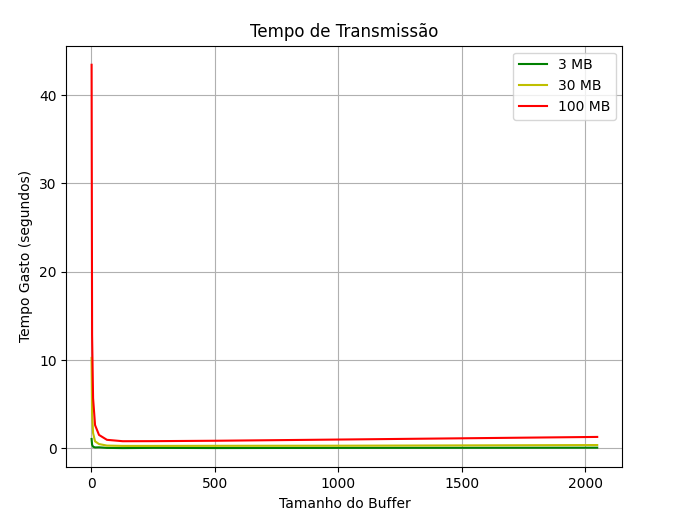
\includegraphics[width=0.85\textwidth]{Images/time.png}
    \caption{Gráfico comparativo do tempo de transmissão}
    \label{fig:exampleFig1}
\end{figure}
\begin{figure}[H]
    \centering
    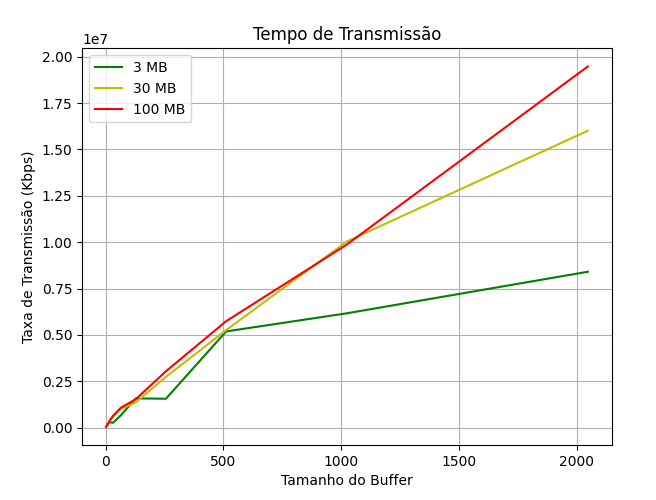
\includegraphics[width=0.85\textwidth]{Images/rate.png}
    \caption{Gráfico comparativo da taxa de transmissão}
    \label{fig:exampleFig2}
\end{figure}

Nas Tabelas \ref{tab:exampleTab1}, \ref{tab:exampleTab2} e \ref{tab:exampleTab3}, são apresentadas as métricas brutas obtidas nos testes realizados:

\begin{table}[H]
    \centering
    \caption{Métricas obtidas nos testes com arquivos de 3 MB}
    \vspace{0.2cm}
    \label{tab:exampleTab1}
    \begin{tabular}{c|c|c}
        \vspace{0.2cm}
        \textbf{Tamanho do Buffer (B)} & \textbf{Taxa de Transmissão (Kbps)} & \textbf{Tempo Total (s)}\\
        2 & 45476,94 & 1,058\\
        4 & 80976,67 & 0,401\\
        8 & 161368,36 & 0,176\\
        16 & 287237,03 & 0,096\\
        32 & 265458,71 & 0,11\\
        64 & 655793,7 & 0,047\\
        128 & 1579705,18 & 0,023\\
        256 & 1559720,75 & 0,047\\
        512 & 5188823,98 & 0,028\\
        1024 & 6165063,97 & 0,048\\
        2048 & 8406721,68 & 0,07
    \end{tabular}
\end{table}

\begin{table}[H]
    \centering
    \caption{Métricas obtidas nos testes com arquivos de 30 MB}
    \vspace{0.2cm}
    \label{tab:exampleTab2}
    \begin{tabular}{c|c|c}
        \vspace{0.2cm}
        \textbf{Tamanho do Buffer (B)} & \textbf{Taxa de Transmissão (Kbps)} & \textbf{Tempo Total (s)}\\
        2 & 46975,68 & 10,238\\
        4 & 83176,28 & 3,901\\
        8 & 164777,43 & 1,725\\
        16 & 352121,73 & 0,785\\
        32 & 607541,81 & 0,48\\
        64 & 1003639,5 & 0,306\\
        128 & 1363187,58 & 0,27\\
        256 & 2735397,89 & 0,27\\
        512 & 5262338,96 & 0,28\\
        1024 & 10035287,11 & 0,294\\
        2048 & 16010119,24 & 0,368
    \end{tabular}
\end{table}

\begin{table}[H]
    \centering
    \caption{Métricas obtidas nos testes com arquivos de 100 MB}
    \vspace{0.2cm}
    \label{tab:exampleTab3}
    \begin{tabular}{c|c|c}
        \vspace{0.2cm}
        \textbf{Tamanho do Buffer (B)} & \textbf{Taxa de Transmissão (Kbps)} & \textbf{Tempo Total (s)}\\
        2 & 36897,98 & 43,45\\
        4 & 84456,54 & 12,807\\
        8 & 167056,68 & 5,67\\
        16 & 351025,27 & 2,625\\
        32 & 642762,61 & 1,513\\
        64 & 1068174,35 & 0,959\\
        128 & 1532469,57 & 0,802\\
        256 & 3037892,07 & 0,856\\
        512 & 5741720,69 & 0,996\\
        1024 & 9867997,07 & 1,287\\
        2048 & 19474089,03 & 1,686
    \end{tabular}
\end{table}

\section{Limitações}

Algumas das limitações encontradas nos testes realizados foram percebidas quando se tentava utilizar \emph{buffers} com capacidade de 4096 \emph{Bytes} ou superior. Também é uma limitação conhecida, a impossibilidade de utilizar o \emph{buffer} cuja capacidade é a mínima disponível (1 \emph{Byte}). Nestes casos, foram observados erros no processo de envio dos arquivos para o cliente por parte do servidor, apresentando mensagens de erro como: \emph{connection reset by peer} e \emph{broken pipe}. O resultado obtido destas execuções (arquivo recebido pelo cliente) era um arquivo de saída (\emph{output.txt}) parcialmente preenchido, o que levou ao descarte das métricas obtidas para tais tamanhos de \emph{buffer}.

\section{Compilação e Execução}

\noindent Para compilar os programas, tanto no lado do cliente, quanto no lado do servidor, basta executar o seguinte comando via terminal:

\begin{center}
    \boxed{\textbf{\large{make}}}
\end{center}

\noindent Na execução, basta executar o seguinte comando via terminal (válido para ambos):

\begin{center}
    \boxed{\textbf{\large{make run}}}
\end{center}

Deve-se atentar à execução do servidor primeiro, para então a conexão TCP ocorrer de forma correta. Além disso, os parâmetros de execução podem e devem ser alterados nos arquivos \emph{Makefile}, alterando o tamanho do \emph{buffer}, nome do arquivo e número de porta, se necessário. Os arquivos presentes no diretório \emph{files} são exibidos na Tabela \ref{tab:exampleTab4}:

\begin{table}[H]
    \centering
    \caption{Arquivos presentes no diretótio \emph{files}}\vspace{0.3cm}
    \label{tab:exampleTab4}
    \begin{tabular}{c|c}
     \textbf{30 MB} & \textbf{3 MB}\\
     524.txt & 644.txt
    \end{tabular}
\end{table}

Também é possível gerar seus próprios arquivos utilizando o \emph{script Python} presente no diretório \emph{aux}. Basta passar o tamanho do arquivo (em MB) no código fonte, e então gerar o arquivo correspondente com nome gerado aleatoriamente executando:

\begin{center}
    \boxed{\textbf{\large{python3 file\_generator.py}}}
\end{center}

\section{Considerações Finais}

Neste trabalho, foi construído a estrutura da comunicação entre um par (\emph{Cliente-Servidor}) para o envio de requisições (nome do arquivo) e respostas (dados do arquivo) seguindo o protocolo de operação no enunciado. Portanto, o objetivo principal era tentar compreender de forma mais clara, como ocorrem os processos de comunicação e transmissão de dados na camada de aplicação e de transporte, além de observar como a execução deste par se comporta, a medida que ser variavam o tamanho dos arquivos e a capacidade dos \emph{buffers}.

Com este exemplo didático, podemos observar de forma nítida, a complexidade por trás da transmissão de dados, mesmo que em volume pequeno, que podem ser requisitados de forma constante em quaisquer redes de computadores, sejam estas locais, regionais, ou globais como a \emph{internet}. 

\section*{Referências}

\begin{itemize}
    \item recv: Connection reset by peer: \url{https://stackoverflow.com/questions/13736064/recv-connection-reset-by-peer};
    \item C library function - fprintf(): \url{https://www.tutorialspoint.com/c_standard_library/c_function_fprintf.htm};
    \item Data Types in C: \url{https://www.geeksforgeeks.org/data-types-in-c/};
    \item How to use gettimeofday function in C language?: \url{https://linuxhint.com/gettimeofday_c_language/};
    \item Setting Decimal Precision in C Language: \url{https://linuxhint.com/setting_decimal_precision_c_-language/};
    \item Material disponível no portal didático na disciplina de Redes de Computadores I.
\end{itemize}

\end{document}